\chapter{Results}

This chapter presents the findings of the experiments conducted in this masters thesis. The chapter is divided into two sections.
The first section presents the results of\method{1}, the second section presents the results of \method{2},
 where both methods will be evaluated in context of both Gaussian VAEs and VQ-VAEs.

\section{Results of \method{1}}

In this section, I will present the results of \method{1} on both Gaussian VAEs and VQ-VAEs.

\subsection{Results on Gaussian VAEs}

\begin{figure}[H]
    \centering
    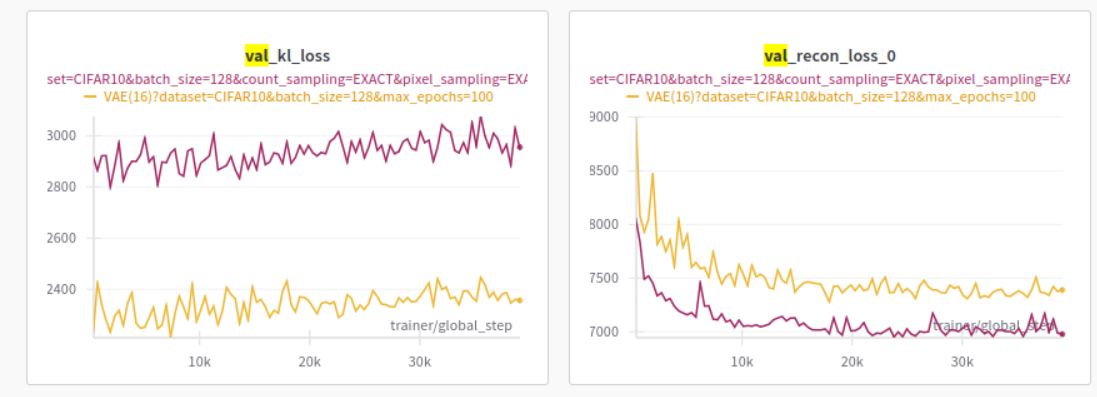
\includegraphics[width=0.8\textwidth]{figures/SCVAE2D_16_CIFAR10.png}
    \caption{KL divergence of the latent space of the Gaussian VAEs.}
    \label{fig:kl_divergence_gaussian_vae}
\end{figure}

\subsubsection{Exact same sampling}

\subsubsection{Uniform sampling}

\subsection{Results on VQ-VAEs}

\subsubsection{Exact same sampling}

\subsubsection{Uniform sampling}


\section{Results of \method{2}}

In this section, I will present the results of \method{2} on both Gaussian VAEs and VQ-VAEs.

\subsection{Results on Gaussian VAEs}

\subsubsection{Uniform random sampling}

\subsubsection{Gaussian sampling}

\subsection{Results on VQ-VAEs}

\subsubsection{Uniform random sampling}

\subsubsection{Gaussian sampling}


